%-%-%-%-%-%-%-%-%-%-%-%-%-%-%-%-%-%-%-%-%-%-%-%-%-%
% EE531: laboratório de Eletrônica Básica I       %  
% Experimento 2: Diodos                           %
% Data:20/08/2010                                 %
% Unicamp,Campinas,São Paulo,Brasil               % 
% Grupo:                                          %
%       - Daniel Lins Mattos                      %
%       - Raquel Mayumi Kawamoto                  %
%       - Tiago Chedraoui Silva                   % 
%-%-%-%-%-%-%-%-%-%-%-%-%-%-%-%-%-%-%-%-%-%-%-%-%-%
%\documentclass[letter]{article}  % formato impressao IC
\documentclass[a4paper]{article} % formato impressao FEEC

%%% fontes %%%
\usepackage[T1]{fontenc}
\usepackage[brazil]{babel}    % dá suporte para os termos na língua portuguesa do Brasi
\usepackage[utf8]{inputenc}   % acentuação
\usepackage{ae,aecompl,aeguill}       % pdfs mais bonitos =)

%%% outros %%%
\usepackage{multirow}
\usepackage{textcomp}
\usepackage{color}       
\usepackage{indentfirst}      % retira padrao americano de paragrafos
\usepackage{multicol}   
\usepackage[linkbordercolor={1 1 1},urlcolor=black,colorlinks=true]{hyperref} % links
\usepackage{subfig}
\usepackage[letterpaper]{geometry}
\geometry{verbose,lmargin=3cm,rmargin=3cm}

% circuito eletrico
\usepackage{electComp}
\usetikzlibrary{decorations,decorations.pathmorphing,decorations.pathreplacing}
\usepackage{verbatim}
\usepackage{pstricks}
\usepackage{boxdims}

\setcounter{tocdepth}{0}

\renewcommand{\thefigure}{\thesection.\arabic{figure}}

\date{Setembro 10, 2010}
% Capa estilizada %
\newcommand*{\titleTMB}{\begingroup \centering \settowidth{\unitlength}{\LARGE EE531} {\large\scshape EE531 - Turma S}\\[0.2\baselineskip] \rule{11.0cm}{1.6pt}\vspace*{-\baselineskip}\vspace*{2pt} \rule{11.0cm}{0.4pt}\\[\baselineskip] {\LARGE  Diodos}\\\vspace*{\baselineskip}  {\itshape Laboratório de Eletrônica Básica I - Segundo Semestre de 2010}\\ \rule{11.0cm}{0.4pt}\vspace*{-\baselineskip}\vspace{3.2pt} \rule{11.0cm}{1.6pt}\\[\baselineskip] {\large\scshape Professor: José Cândido Silveira Santos Filho}\par \vfill {\normalsize   \scshape 
    \begin{center} 
      \begin{tabular}{  l  l  p{5cm} } 
 	Daniel Lins Mattos & RA: 059915\\
        Raquel Mayumi Kawamoto & RA: 086003\\
        Tiago Chedraoui Silva  & RA: 082941\\
      \end{tabular} \end{center}
    \itshape 10 de setembro de 2010    }\\[\baselineskip] \vspace{3.2pt} \endgroup}


\begin{document}
\titleTMB 
\newpage


Este experimento visa o estudo do diodo semicondutor, elemento não-linear
fundamental de um circuito. Assim como um resistor, o diodo tem dois terminais; mas,diferentemente do resistor, o qual tem uma relação linear (direta) entre a corrente que circula por ele e a tensão aplicada, o diodo tem uma característica i-v não-linear.
      Portanto, para um melhor entendimento do funcionamento e das características de um diodo, este experimento trata da aplicação mais comum do diodo, o projeto de circuitos retificadores (o qual converte ca em cc).

        Assim como no primeiro experimento, foi utilizado o protoboard para a montagem dos
circuitos. Foi necessário, ainda, a utilização de oito diodos 1N4001 ou 1N4002, dois diodos
1N4148, três capacitores eletrolíticos $100\mu$F,  um amplificador operacional 741, dois resistores
de $10k\Omega$, um resistor de $1k\Omega$ e um tranformador de 110 $V_{ac}$,9 $V_{ac}$.


\section*{Parte Experimental}
%\begin{enumerate}
%\item
\section{Amplificador Operacional}
 \setcounter{figure}{0}

Um amplificador operacional amplifica uma diferença potencial elétrica presente às suas entradas sendo uma designado por terminal inversor(-) e a outra por terminal não inversor(+).
Caso o amplificador operacional seja ideal, algumas de suas características são possuir impedância de entrada infinita, impedância de saída nula e ganho infinito em malha aberta.

 Para esta parte inicial do experimento, o circuito da figura \ref{circ:1} --- composto de um amplificador operacional 741, um resistor (R$_i$) de $1k\Omega$, e dois diodos 1n4148 (D$_1$ e D$_2$) --- é montado e o canal um do osciloscópio é colocado entre D$_1$ e R$_i$ e o canal dois na saída do amplificador operacional. 

Além disso, o gerador de funções é ajustado para produzir um sinal de tensão com sua forma de onda triangular, com amplitude 10$V_{pp}$, com offset de $5V$, frequência de $10kHz$ e simetria de 50\%. 

O circuito produzido é conhecido como amplificador inversor, pois o sinal de saída tem uma diferença de fase de $180^{\circ}$ em relação ao sinal de entrada, o que implica em uma mudança de sinal entre a entrada e saída, se uma é positiva a outra é negativa. Logo é importante que a onda gerada seja positiva, pois, caso fosse negativa, o diodo $D_2$ bloquearia o sinal de realimentação negativa, que é utilizado para impedir que o amplificador sature. Portanto, se existisse um entrada negativa, o amplificador saturaria.

\vspace{3mm}
\begin{figure}[h]
\centerline{\input circ1.tex}
\caption{Circuito para caracterização V versus I do diodo \label{circ:1}}
\end{figure}

Supondo que o amplificador operacional seja ideal, nenhuma corrente de entrada é drenada, ou seja, a corrente $i$ caracterizada em $D_1$ e $R_i$ é a mesma que em $D_2$. Além disso, a tensão entre o terminal de saída e o terra é equivalente a $A(v_2-v_1)$, sendo o ganho $A$ idealmente infinito. Logo, tem-se que:
\begin{equation}
\frac{V_D}{A}=(v_2-v_1)\approx0
\end{equation}

Como $v_1=0$ temos que $v_2=0$, assim:
\begin{equation}
i=\frac{V_{CH2}}{R_{i}}\\
\end{equation}

A partir dos dados obtemos $V_{CH2}=8,72V$, logo $I_D$ vale $8,72mA$.

Utilizando o canal 1, tem-se que:  

\begin{equation}
V_D=-V_{CH1}\\
\end{equation}


Utilizando o recurso Time Base X-Y do osciloscópio, obtemos uma curva caracterísica (V versus I) do diodo presente na figura \ref{fig:q1-curva2} cuja escala do eixo $V_D$ vale $500mV$/divisão. Portanto, pode-se observar através do gráfico que o diodo em condução direta apresenta um queda de tensão de aproximadamente $0,7V$ e, para tensões inferiores a $0,7V$, o diodo não conduz e para tensões superiores passa a conduzir corrente.    
\begin{figure}[h]
\begin{centering}
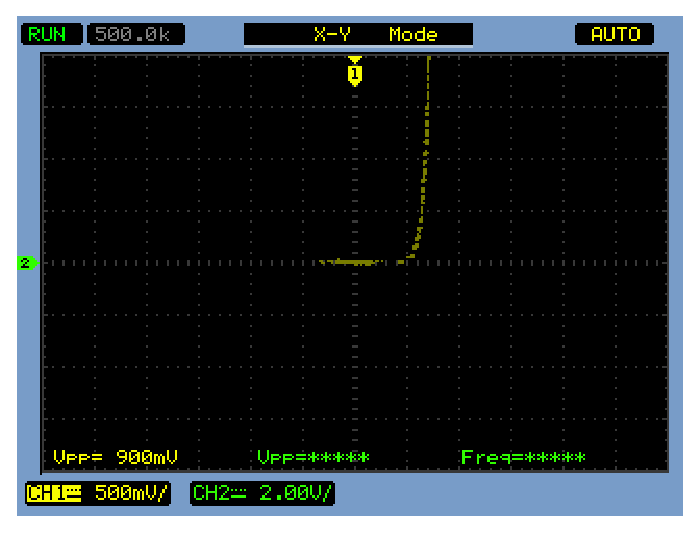
\includegraphics[scale=0.5]{Imagens/3.1/NewFile0} \caption{Curva característica V versus I do diodo  \label{fig:q1-curva2}}
\par\end{centering}
\end{figure}


Como outra caracterísca dos diodos, existe o \textit{tempo de recuperação inverso $t_{rr}$}, que é o o tempo decorrido para o diodo deixar de conduzir após a mudança de polarização de direta para inversa. Ou seja, apesar do sinal de entrada passar do mínimo para o máximo e vice-versa, há um certo atraso para que essa transição ocorra causado pela característica do sistema de conservar suas propriedades. Para um diodo ideal esse tempo de atraso seria nulo.

Para analizar esse tempo, trocou-se no circuito o diodo 1N4148 --- diodo de pequenos sinais cujo tempo de recupeção inverso está na faixa dos nanosegundos ---  pelo 4001, que possui um tempo de recuração inverso na faixa nos microsegundos. Devido a esse atraso, a curva de histerese pode ser vista, pois quando o sinal está no máximo, devido às características de conservação, a queda de tensão gera a parte superior da curva da figura \ref{fig:q1-his} ao manter por mais tempo um valor mais alto de sinal e, quando está no valor mínimo, a transição gera a parte inferior da curva de histerese, ao manter um valor mais baixo por mais tempo. Variando a frequência do circuito, quanto menor a frequência maior é a área da curva, quanto maior a frequência sua área diminui.


\begin{figure}[h]
\begin{centering}
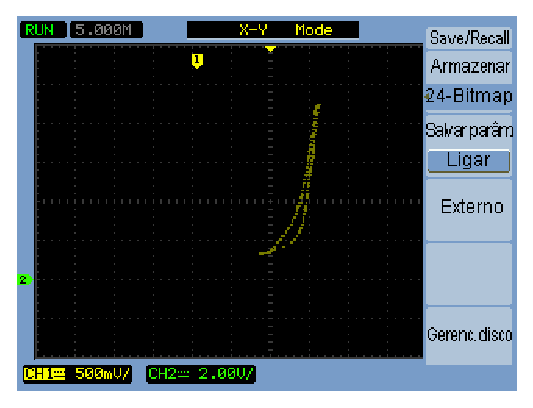
\includegraphics[scale=0.7]{Imagens/3.1.opcional/opcio} \caption{Curva de histerese \label{fig:q1-his}}
\par\end{centering}
\end{figure}

\renewcommand{\thefigure}{\thesubsection.\arabic{figure}}

\newpage
\section{Circuitos retificadores}
 \setcounter{figure}{0}
O circuito retificador é uma aplicação fundamental do diodo, que faz uso intenso da curva não-linear i-v. Este circuito consiste em um diodo $D$ e um resistor $R$ conectados em série. Supondo uma tensão de entrada senoidal  $v_1$ e um diodo ideal, durante os semicilos positivos da entrada senoidal, a tensão positiva  $v_1$ faz com que a corrente circule pelo diodo no sentido direto. Como a tensão no diodo será muito pequena, idealmente zero, a tensão de saída  $v_0$ será igual a tensão de entrada      $v_1$     . Durante os semiciclos negativos de    $v_1$    , o diodo não conduzirá. Portanto,   $v_0$     será zero. A figura 2.1 ilustra os circuitos em cada semiciclo de   $v_1$  e as formas de ondas de saída  $v_0$      .
        Observa-se que, enquanto $v_1$ alterna em polaridade e tem um valor médio zero, $v_0$ é unidirecional e tem um valor médio finito, ou uma componente cc. Portanto, o circuito retificador retifica o sinal, sendo por isso denominado de retificador. Ele pode ser usado para gerar cc a partir de ca.
         Para este experimento foram estudados dois tipos de circuitos retificadores: retificador de meia onda e retificador de onda completa tipo ponte.
      
\subsection{Retificador de meia onda}
         Inicialmente foi montado no protoboard o circuito da figura \ref{fig:ret-circ1} circuito retificador de meia onda que consiste em um diodo de retificação (diodo 1N4001) e um resistor (de valor $10k\Omega$) conectados em série, alimentados por um transformador de $110V_{ac}$.
         Um circuito retificador de meia onda utiliza metade dos semiciclos da senóide de entrada. Supondo um diodo ideal, durante os semiciclos positivos da entrada senoidal, a tensão positiva $V_s$ faz com que a corrente circule pelo diodo no sentido direto. Segue que a tensão no diodo será muito pequena idealmente zero. Portanto, a tensão de saída $V_0$ será igual à tensão de entrada $V_s$. Por outro lado, durante os semiciclos negativos de $V_s$, o diodo não conduzirá, sendo a tensão de saída igual a zero. Enquanto $V_s$ alterna em polaridade e tem um valor médio zero, a tensão de saída é unidirecional e tem um valor médio finito, ou uma componente cc.
         Como o diodo do circuito da figura \ref{fig:ret-circ1} não é ideal, pode-se escrever:
     
\begin{equation}
  v_0=0,       v_s<V_{DO}
\end{equation}
\begin{equation}
v_0=\frac{R}{R+r_D}v_s -V_{DO}\frac{R}{R+r_D},      v_s \geq V_{DO}
\end{equation}


    Em que   $V_{DO}$     e $r_D$ são, respectivamente, a tensão e a resistência do diodo.
         Em muitas aplicações tem-se  $r_D \ll R$           e a segunda equação pode ser simplificada para:
\begin{equation}
v_0 \cong v_s-V_{DO}
\end{equation}


         Um dos principais parâmetros de um diodo no projeto de retificadores é a tensão de pico inversa (\textit{peak inverse voltage} – PIV) que o diodo deve ser capaz de suportar sem atingir a
tensão de ruptura, determinada pelo maior valor de tensão inversa que pode aparecer no diodo. Pelo circuito da figura  \ref{fig:ret-circ1} observa-se que, quando $v_s$ é negativo, o diodo corta e   $v_0$      é
igual a zero. Portanto, conclui-se que a PIV é igual ao valor de pico $v_s:PIV=V_s$.




\begin{figure}[h!]
\begin{centering}
\subfloat[]{
%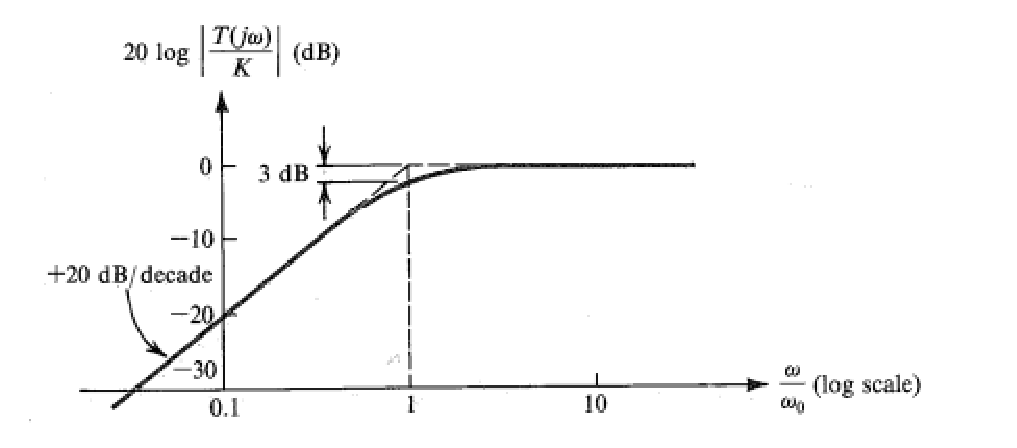
\includegraphics[scale=0.45]{Imagens/mag_h.eps}
\input circ2.tex
 \label{fig:retmeia-circ1(a)}
}

\subfloat[]{
\includegraphics[scale=0.45]{Imagens/3.3.1ret_meia_onda/311}
 \label{fig:retmeia-circ1(b)}
}
\subfloat[]{
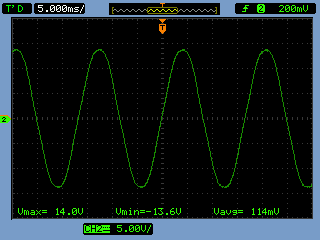
\includegraphics[scale=0.45]{Imagens/3.3.1onda_completa/p1q3}
\label{fig:retmeia-circ1(c)}
}
\subfloat[]{
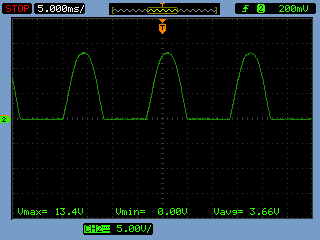
\includegraphics[scale=0.45]{Imagens/3.3.1onda_completa/p2q3}
\label{fig:retmeia-circ1(d)}
}
\par\end{centering}


\caption{(a) Circuito Retificador de Meia Onda. (b)  Formas de onda de entrada e saída.(c) Forma de onda no nó 1 (d) Forma de onda no nó 2 \label{fig:ret-circ1}.}

\end{figure}

\newpage
          Fazendo-se a análise do esquemático da figura  \ref{fig:retmeia-circ1(a)}, pode-se ver o funcionamento de um retificador de meia onda a partir das formas de ondas capturadas no osciloscópio dos nós 1 e 2 do circuito da figura  \ref{fig:retmeia-circ1(b)}. Os nós 1 e 2 correspondem, respectivamente, ao canal 1(CH1) e ao canal 2 (CH2) do osciloscópio. Nos semiciclos positivos, como o diodo encontra-se em curto, irá passar corrente pelo circuito, criando uma tensão de saída no resistor. Os diodos introduzem perdas na tensão final de modo que a tensão de saída tende a $v_0=v_s-V_{DO}$. Pode-se verificar pela figura  \ref{fig:retmeia-circ1(b)} que a máxima tensão de saída do circuito é de   $13.4 Volts$. Portanto,    $V_{DO}= 0.8V $. Nos semiciclos negativos, o diodo não conduz, portanto a tensão de saída é zero.


Analisando a figura \ref{fig:retmeia-circ1(b)},  \ref{fig:retmeia-circ1(c)}, \ref{fig:retmeia-circ1(d)} obtemos, os valores das ondas presentes na tabela \ref{tab:ret_mei_onda}. Teoricamente no nó 2 deveria obter-se $V_{min}=0V$ e $v_0=13,4V$, ambos os valores condizem com os valores encontrados.

    
\begin{table}[h!]
\begin{centering}
\begin{tabular}{|c|c|c|c|}
\cline{2-4} 
\multicolumn{1}{c|}{} & $V_{min}$ & $V_{max}$ & $V_{avg}$\tabularnewline
\hline 
Nó 1 & $-13,6V$ & $14,2V$ & $114mV$\tabularnewline
\hline 
Nó 2 & $0V$ & $13,4V$ & $3,66V$\tabularnewline
\hline
\end{tabular}
\par\end{centering}

\caption{Valores de máximo, mínimo e média das ondas nos nós 1 e 2.}
\label{tab:ret_mei_onda}
\end{table}



 \subsection{ Retificador de Onda Completa tipo Ponte}
         Foi montado no protoboard o circuito da figura \ref{fig:ret-circ2} circuito retificador de onda completa tipo ponte que consiste em quatro diodos de retificação $D$ (diodo 1N4001) e um resistor $R$    (de valor $10k\Omega$) dispostos conforme indica a figura \ref{fig:ret-circ2}, alimentados por um transformador de $110V_{ac}$.
         O circuito retificador em ponte opera da seguinte maneira: durante os semiciclos positivos da tensão de entrada $v_s$, é positiva e a corrente é conduzida pelo diodo $D_1$, resistor $R$ e diodo $D_2$. Enquanto isso, os diodos  $D_3$      e $D_4$   estarão inversamente polarizados. Durante os semiciclos negativos da tensão de entrada, a tensão $v_s$ no secundário será negativa e, portanto,  $-v_s$     será positiva, forçando a corrente a circular por $D_3$ , $R$ e $D_4$ . Enquanto isso, os diodos $D_1$ e $D_2$   estarão inversamente polarizados.
         Deve ser observado que durante ambos os semiciclos, a corrente circula por $R$ no mesmo sentido (do ponto 3 para o ponto 0) e então   $v_o$    será sempre positiva.
         Para determinar a tensão de pico inversa (PIV) de cada diodo, considera-se o circuito durante os semiciclos positivos. A tensão inversa sobre o diodo $D_3$ pode ser estabelecida pela malha formada por $D_3$, R e $D_2$         como  $v_{D3}(inverso)v_o+v_{D2}(direto)$. Logo, o valor máximo de $v_{D3}$     ocorre no pico de $v_o$    e é dado por:
                                    
\begin{equation}
PIV=V_S-2V_D+V_D=V_S-V_D
\end{equation}

Analisando as figuras \ref{fig:ret-circ2(b)}, \ref{fig:ret-circ2(c)}, \ref{fig:ret-circ2(d)} obtemos, os valores das ondas presentes na tabela \ref{tab:ret_tot_onda}. Teoricamente no nó 1,2 e 3 deveria obter-se $V_{min}=0V$, porém, no nó 3 deveria-se obter  $v_{max}=12,0V$, um diferença de 7,7\% com o teórico.


\begin{table}[h!]
\begin{centering}
\begin{tabular}{|c|c|c|c|}
\cline{2-4} 
\multicolumn{1}{c|}{} & $V_{min}$ & $V_{max}$ & $V_{avg}$\tabularnewline
\hline 
Nó 1 & $-400mV$ & $13,6$ & $3,96V$ \tabularnewline
\hline 
Nó 2 & $-400mV$ & $13,6V$ & $3,98V$\tabularnewline
\hline 
Nó 3 & $-200mV$ & $13,0V$ & $8,25V$\tabularnewline
\hline
\end{tabular}
\par\end{centering}

\caption{Valores de máximo, mínimo e média das ondas nos nós 1,2 e 3 referentes ao circuito  \ref{fig:ret-circ2(a)}.}

\label{tab:ret_tot_onda}
\end{table}


\begin{figure}[h!]
\begin{centering}
\subfloat[]{
\input circ3.tex
 \label{fig:ret-circ2(a)}
}
\par\end{centering}
\subfloat[]{
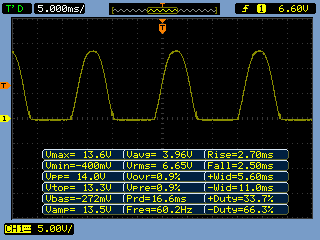
\includegraphics[scale=0.45]{Imagens/3.3.1onda_completa/no1}
 \label{fig:ret-circ2(b)}
}
\subfloat[]{
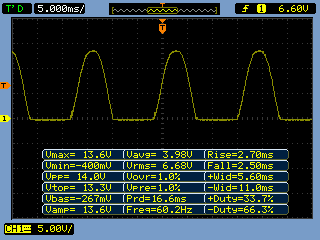
\includegraphics[scale=0.45]{Imagens/3.3.1onda_completa/no2}
\label{fig:ret-circ2(c)}
}
\subfloat[]{
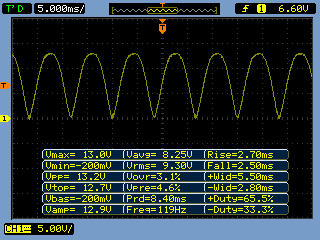
\includegraphics[scale=0.45]{Imagens/3.3.1onda_completa/no3}
\label{fig:ret-circ2(d)}
}

\caption{(a) Circuito Retificador de Onda Completa tipo Ponte. (b) Forma de onda
no ponto do nó 1. (c) Forma de onda no ponto do nó 2. (d) Forma de onda no ponto do nó 3. \label{fig:ret-circ2}}
\end{figure}




Posteriormente, realizando uma análise dos circuitos  \ref{fig:ret-circ2(a)} e \ref{fig:retmeia-circ1(a)}, tem-se que o PIV do retificador meia onda vale $14,2V$ e o da onda completa $12,8V$. O retificador de completa tem PIV menor, sendo devido a diferença do diodo.


\newpage
Portanto,comparando os dois circuitos,um circuito retificador de onda completo possui um $V_{avg}$ maior que um circuito retificador de meia onda, já que utiliza ambos semiciclos da senóide de entrada, resultando em uma saída cuja frequência é maior, ou seja dentro de um mesmo intervalo a onda retificadora apresenta o dobro de picos que o retificador de meia onda. Outra diferença é o valor do PIV, que no circuito retificador de meia onda é maior que no de onda completa. 


    Com o objetivo de montar uma fonte de tensão DC não regulada, introduziu-se o capacitor eletrolítico de  $100\mu$F entre os nós 3 e 0 da Figura \ref{fig:ret-circ2}, ou seja, o capacitor é incluído em paralelo com o resistor de carga. Dessa forma, obteve-se um circuito retificador com capacitor de filtro (o retificador de pico).
         O circuito retificador de pico opera da seguinte maneira: inicialmente, o capacitor está descarregado; durante o primeiro semiciclo da tensao do secundário, o diodo está conduzindo permitindo que o secundário carregue o capacitor até a tensão de pico; logo após, no semiciclo negativo, o diodo pára de conduzir (o que significa uma chave aberta) e neste estágio, como o capacitor tem uma tensão $V_p$, ele polariza o diodo inversamente e começa a descarregar-se no resistor de carga. Deve ser considerado a constante de tempo de descarga do capaciotr, que é função do resistor $R$ e do capacitor $C$. Esta constante deve ser bem maior do que o período $T$ do sinal de entrada. Dessa forma, o capacitor só se descarregará um pouco até o próximo ciclo.

A figura \ref{fig:cap-ret} ilustra a forma de onda do retificador de pico.

\begin{figure}[h!]
\begin{centering}
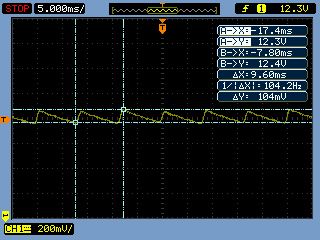
\includegraphics[scale=0.7]{Imagens/3.3.4capacitor_paralelo/3cap} \caption{Forma de onda da tensão no capacitor do retificador de pico. \label{fig:cap-ret}}
\par\end{centering}
\end{figure}


De acordo com a figura \ref{fig:cap-ret} $V_r$ vale $104mV$. Para uma comparação teórica, temos através da equação (8) que $V_r$ depende de $V_p$ ($12,3V$) e inversamente do capacitor ($100\mu$F), resistor ($10k\Omega$), frequência ($119Hz$).Logo, $V_r$ teórico vale $103mV$.  

\begin{equation}
V_r = \frac{V_p} {fCR}
\end{equation}

Portanto, o valor obtido difere em 1\% do valor teórico.

\renewcommand{\thefigure}{\thesection.\arabic{figure}}

\section{Duplicador de Tensão}

No circuito denominado Duplicador de Tensão o diodo $D_1$ conduz quando a tensão de entrada é positiva, carregando o capacitor $C_1$. Esse capacitor terá uma tensão igual a $V_p$ ao carregar-se. Quando a tensão de entrada é negativa, o diodo $D_2$ conduz, carregando o capacitor $C_2$ com a mesma polarização de $C_1$, também com tensão $V_p$. Em regime permanente, a queda de tensão nos capacitores será muito pequena comparada às amplitudes dos sinais, resultando em uma saída entre nós 1 e 2 de aproximadamente $2V_p$, podendo chamar o circuito de Duplicador de Tensão.

A forma de onda na entrada, como foi pedido no item, está ilustrada nas Figuras \ref{fig:dob}, medidas no canal 1.
É uma onda quadrada de aproximadamente $10 V_{pp}$, frequência de $1kHz$ e duty cycle de aproximadamente
50\% para a parte positiva e negativa do sinal. A ponta de prova do canal 2 foi colocada no nó 1 e a ponta do canal 1 foi colocada no nó 2, a fim de medir
a diferença de potencial entre os dois nós, que é a tensão de saída do circuito. A
mesma é, como esperávamos, uma tensão contínua, aproximadamente igual a
duas vezes a tensão de pico da onda quadrada de entrada.
Isso é evidenciado na figura \ref{fig:dob-no12}, onde é possível observar claramente uma diferença de potencial de aproximadamente $2V_p$ entre os nós 1 e 2. A discrepância entre a tensão contínua de saída e $2V_p$ é devido a um pequeno descarregamento dos capacitores, o que fica menos significativo quando aumenta-se a frequência da onda de entrada.



 \setcounter{figure}{0}
\vspace{3mm}
\begin{figure}[h]
\centerline{\input circ4.tex}
\caption{Duplicador de tensão \label{tab:circ}}
\end{figure}


\begin{figure}[h!]
\begin{centering}
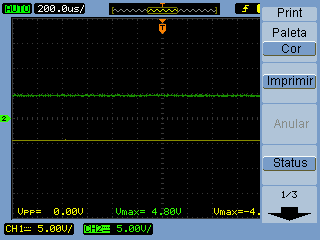
\includegraphics[scale=0.50]{Imagens/3.4duplicador_tensao/423} \caption{Tensão de saída nos nós 1 e 2 \label{fig:dob-no12}}
\par\end{centering}
\end{figure}


\begin{figure}[h!]
\begin{centering}
\par\end{centering}
\end{figure}


\begin{figure}[h!]
\begin{centering}
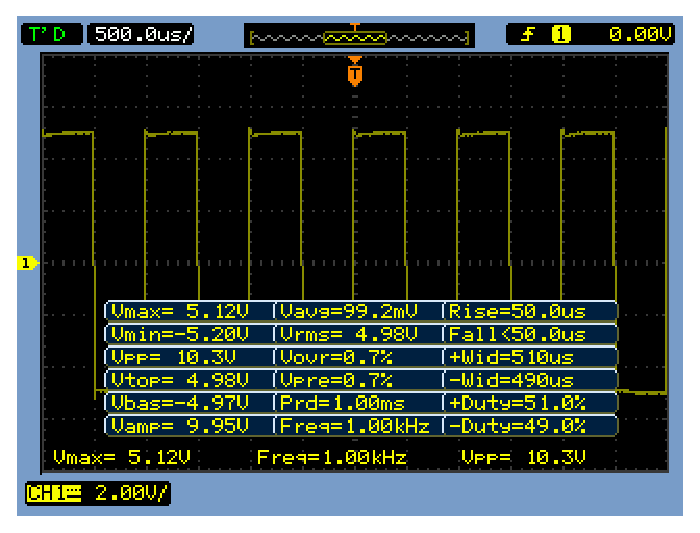
\includegraphics[scale=0.50]{Imagens/3.4duplicador_tensao/Vinmedidas}
\par\end{centering}
\caption{ Medidas da onda de entrada do circuito. \label{fig:dob}}
\end{figure}


\end{document}
